\chapter{绪论}
\thispagestyle{fancy}
\section{研究背景}
根据中国互联网络信息中心的统计\cite{CN12},截至2012年12月底,中国有近半数网民在使用微博,比例达到 48.7\%,较上一年底增长了 296.0\%,相比之下,网络新闻使用率从 2009 年底的 80.1\% 下降至 71.5\%,网民通过互联网获取新闻信息的渠道正向微博发生转移。
   
在中文微博产品中,新浪微博\footnote{http://weibo.com}最具代表性和影响力。和传统社交网站不同,新浪微博上的社交关系以话题为中心,一个社会热点话题往往能在新浪微博上引起广泛的关注和讨论,例如 2012 伦敦奥运会,江南 style,中国好声音等。和话题相关的微博数量,转发量和评论量会在短期内迅速增加,而且会随着话题的发展保持一段时间。不仅如此,这些数据还带有地域性的特征,如话题发生地附近的相关微博数量显著大于地理距离较远的地方。此外,微博中包含的情绪词可以体现出用户对某一话题的态度和情绪。

微博用户在撰写微博时,可以用 Hashtag \cite{hashtag} 表示一个话题,如 “\#雅安地震\#”,新浪微博根据话题的出现次数,可以实时地统计出热点话题; 此外,微话题应用(图 1-1)按照热度(热度由某一话题在近段时间的讨论数及全部讨论数综合计算得出)对话题进行排名,提供话题的简介和相关微博(指出现该话题的微博)。用户可以查询不同时段(一月,一周和24小时内),不同地域和不同分类下(如影视,公益等)的热点话题。在现有的新浪微博平台上,用户可以实时地跟踪热点话题并参与讨论,但是并不能了解话题发展的整体趋势和特征,如和话题相关的微博数随时间的变化趋势,在地域上的分布差异,以及微博中的情绪特征等。

\begin{figure}[t]
\centering
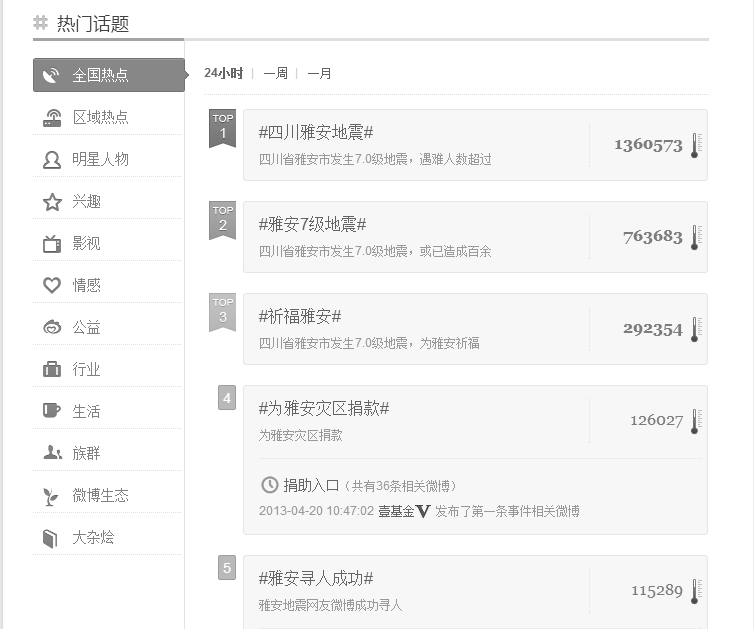
\includegraphics[width=\textwidth, height=0.35\textheight]{weihuati}
图 1-1 新浪微博微话题 
\caption{Sina Weibo Weihuati}
\end{figure}

\begin{figure}[t]
\centering
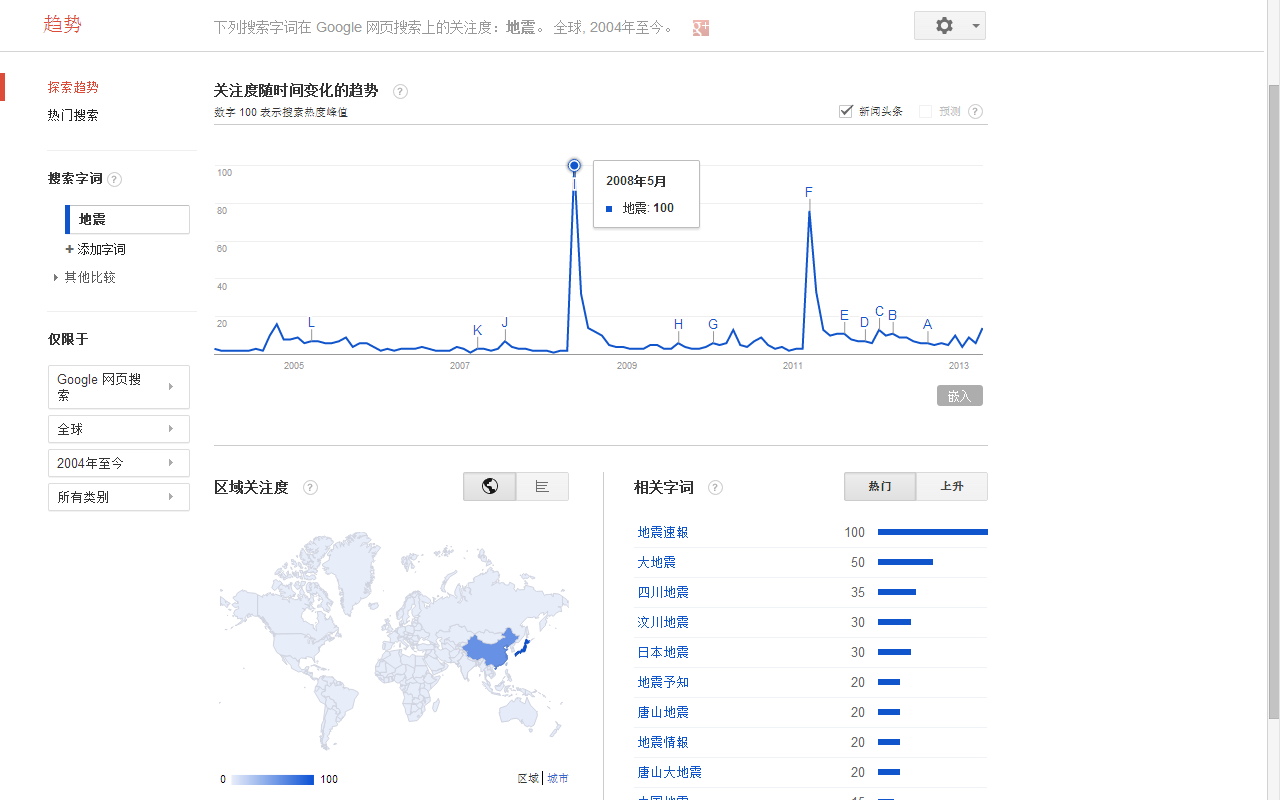
\includegraphics[width=\textwidth, height=0.35\textheight]{google_trends}
\\
图 1-2 谷歌趋势
\caption{Google Trends}
\end{figure}

不仅如此,文字描述对用户而言乏味枯燥,信息的表达效率较低。与之相比,数据可视化技术\cite{perception}借助于图形化手段,清晰有效地传达与沟通信息。Google Trends 通过统计用户的搜索词,用可视化的方式显示其随时间的变化趋势(以月为单位)和地域间搜索次数的差异。通过 Google Trends,用户不再需要在大量的文字中寻找自己感兴趣的信息,而是立即能从图像中识别出来。如图 1-2 所示,在 Google Trends 上搜索“地震”,可以很快地在折线的波峰处找到历年来发生的各次地震事件(最为突出的是汶川地震和福岛地震)。而地图上颜色较深的区域也显示出中国和日本是地震的重灾区。

同样地,将微博数据可视化也能帮助用户迅速地提取信息,发现热点话题,关注社会事件。

本文介绍了 VisualMiner,一个新浪微博热点话题的可视化查询系统。系统对新浪微博数据进行挖掘,将话题的信息按照时间,地域,情绪等维度以可视化的方式呈现在网页端,供用户查询检索。用户看到的不再是单调的文字描述,而是形象化的展示,不再局限于热点事件的一个方面,而是事件的全貌。


\section{论文组织}
本论文分六个章节,具体章节安排如下:
\begin{itemize}
\item 第一章,绪论。介绍论文的研究背景和研究内容
\item 第二章,相关工作。介绍系统使用的 Google App Engine,Hadoop 及 jQuery 等相关平台和框架。
\item 第三章,系统设计。介绍系统的功能设计,界面设计和架构设计。
\item 第四章,系统实现。介绍系统的实现细节,包括数据抓取,数据分析和数据的可视化展示。
\item 第五章,实验结果。介绍系统的实现效果。
\item 第六章,总结和展望。
\end{itemize} 
